\documentclass[12pt,letterpaper,twoside]{article}

\newif\ifsolution\solutiontrue   % Include the solutions
%\newif\ifsolution\solutionfalse  % Exclude the solutions

\usepackage{cme213}
\usepackage{xcolor}
\usepackage{graphicx}

\newcommand{\T}[1]{\text{\texttt{#1}}}
\newcommand{\V}[1]{\text{\textit{#1}}}

\begin{document}

{\centering \textbf{Homework 4: CUDA GPU Matrix Operations\\}}
\vspace*{-8pt}\noindent\rule{\linewidth}{1pt}

Goal of the homework is to implement a finite difference solver for the
2-dim heat equation using CUDA GPU programming.

\paragraph{Problem 1: Implement gpuStencil Global } Idea: parallelize spatial
dimension updates for each time step iteration. One key challenge was to handle
the different border sizes for order inputs of 2, 4 and 8. Kernel logic included
below.

\begin{cpp}
/**
 * Kernel to propagate finite difference grid from the current
 * time point to the next.
 */
template<int order>
__global__
void gpuStencilGlobal(float* next, const float* __restrict__ curr, 
                      int gx, int nx, int ny, float xcfl, float ycfl) {
    
    int borderSize = (int) (order / 2);
    int i = blockIdx.x * blockDim.x + threadIdx.x;
   
    if (i < nx*ny) {
	int x = borderSize + (int) (i / nx);
	int y = borderSize + (i % nx);
        int idx = gx * y + x;   
        next[idx] = Stencil<order>(&curr[idx], gx, xcfl, ycfl);
    
    }
}
\end{cpp}

3D surface plots of temperature on 256 x 256 grid at iterations 0, 1000 and 
2000 respectively, with 8th order. To do this, I used parameter settings of:
order = 8 and nx = ny = 248.

\begin{figure}[h]
    \center
    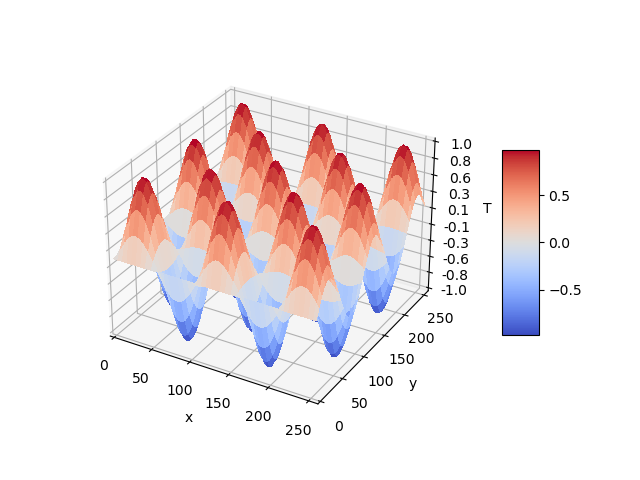
\includegraphics[scale=0.7]{global_0000.png}
    \caption{3D surafce plot of temperature at iteration 0}
\end{figure}

\begin{figure}[h]
    \center
    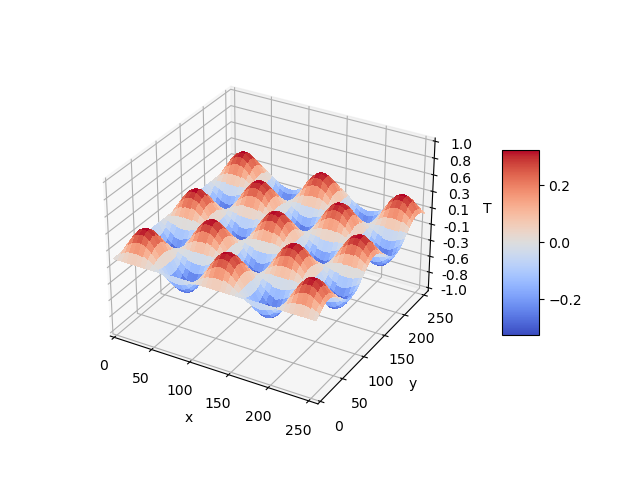
\includegraphics[scale=0.7]{global_1000.png}
    \caption{3D surafce plot of temperature at iteration 1000}
\end{figure}

\begin{figure}[h]
    \center
    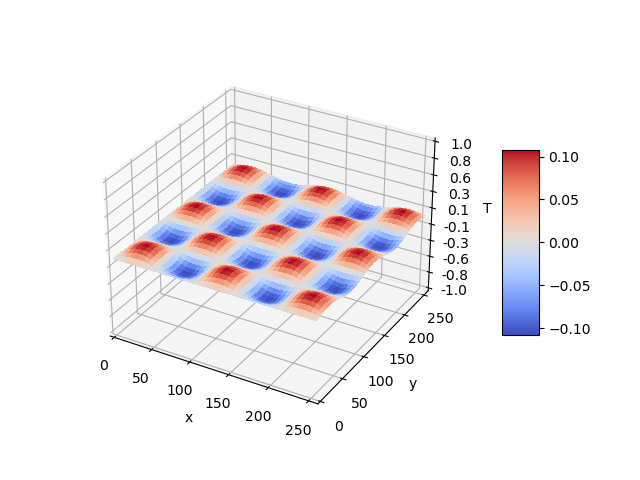
\includegraphics[scale=0.7]{global_2000.png}
    \caption{3D surafce plot of temperature at iteration 2000}
\end{figure}


\paragraph{Problem 2: Implement gpuStencil Block } Idea: ...

...
...

Submission information logs.
\begin{verbatim}
jelc@cardinal2:~$ /afs/ir.stanford.edu/class/cme213/script/submit.py hw3 private/cme213-jelc53/hw3
Submission for assignment 'hw3' as user 'jelc'
Attempt 2/10
Time stamp: 2022-05-01 21:36
List of files being copied:
    private/cme213-jelc53/hw3/main_q1.cu	 [13253 bytes]
    private/cme213-jelc53/hw3/recurrence.cuh	 [1589 bytes]
    private/cme213-jelc53/hw3/pagerank.cuh	 [5894 bytes]
    private/cme213-jelc53/hw3/benchmark.cuh	 [795 bytes]

Your files were copied successfully.
Directory where files were copied: /afs/ir.stanford.edu/class/cme213/submissions/hw3/jelc/2
List of files in this directory:
    main_q1.cu	 [13253 bytes]
    recurrence.cuh	 [1589 bytes]
    pagerank.cuh	 [5894 bytes]
    benchmark.cuh	 [795 bytes]
    metadata	 [137 bytes]

This completes the submission process. Thank you!
    
jelc@cardinal2:~$ ls /afs/ir.stanford.edu/class/cme213/submissions/hw3/jelc/2
benchmark.cuh  main_q1.cu  metadata  pagerank.cuh  recurrence.cuh
\end{verbatim}

\end{document}
